\documentclass[11pt]{article}
\usepackage[usenames]{color} %used for font color
\usepackage{amssymb} %maths
\usepackage{amsmath} %maths

\usepackage[no-math]{fontspec}
\usepackage{unicode-math}
\usepackage{libertinus}

\usepackage{pgf,xcolor}
\definecolor{itwm_blue_04}{HTML}{005A94}
\definecolor{itwm_red}{HTML}{C00000}

\usepackage{tikz}
\usetikzlibrary{shapes.misc, shadows, decorations}
\usetikzlibrary{backgrounds}
\usetikzlibrary{calc}
\usepackage{pgfplots}
\pgfplotsset{compat=newest}
\usepgfplotslibrary{fillbetween}
\usepackage{tikzpagenodes}
\begin{document}
\begin{align*}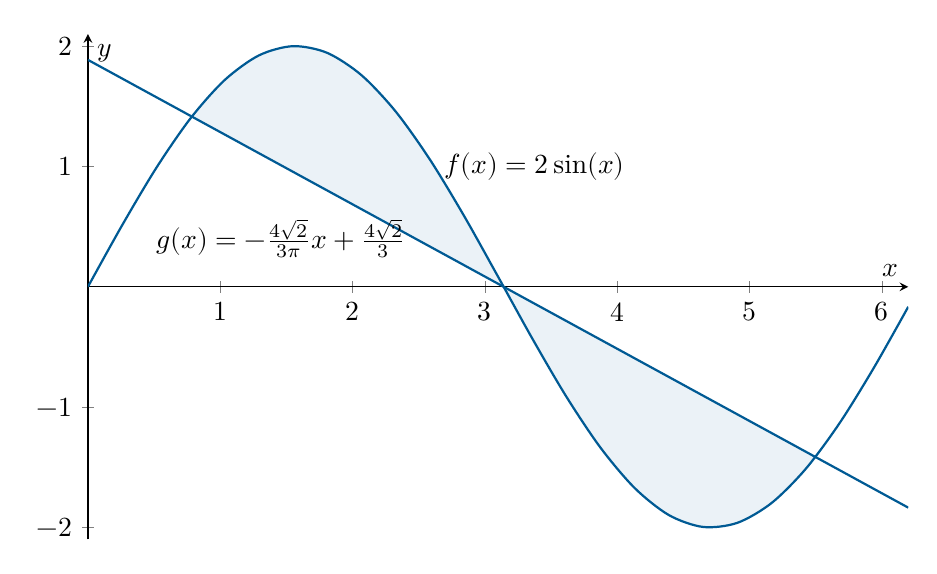
\begin{tikzpicture}
\begin{axis}[
    domain=0:6.2,
    axis lines = center,
    xlabel = {$x$},
    ylabel = {$y$},
    height=8cm, width=12cm, 
    xmin=0, xmax=6.2, ymin=-2.1, ymax=2.1, 
    xtick={0, 1,...,6},
    ytick={-2,-1,...,2}
]
\path [name path=xaxis]
      (\pgfkeysvalueof{/pgfplots/xmin},0) --
      (\pgfkeysvalueof{/pgfplots/xmax},0);
\addplot[draw=itwm_blue_04, smooth, thick, name path=f]{2*sin(deg(x))} node [pos=0.4, right] {$f(x)=2\sin(x)$};
\addplot[draw=itwm_blue_04, smooth, thick, name path=g]{(-4*sqrt(2))/(3*pi)*x + (4*sqrt(2))/(3)} node [pos=0.4, left] {$g(x)=-\frac{4\sqrt{2}}{3\pi}x + \frac{4\sqrt{2}}{3}$};
\addplot[itwm_blue_04!20, opacity=0.4] fill between [of=f and g, soft clip={domain=pi/4:7*pi/4}];
\end{axis}
\end{tikzpicture}
\end{align*}
\end{document}